\documentclass[twoside,11pt]{article}

% Any additional packages needed should be included after jmlr2e.
% Note that jmlr2e.sty includes epsfig, amssymb, natbib and graphicx,
% and defines many common macros, such as 'proof' and 'example'
%
% It also sets the bibliographystyle to plainnat; for more information on
% natbib citation styles, see the natbib documentation, a copy of which
% is archived at http://www.jmlr.org/format/natbib.pdf

\usepackage{jmlr2e}
\usepackage{amssymb}
\usepackage{enumitem}
\usepackage{amsmath}
\usepackage{adjustbox}
\usepackage{caption}
\usepackage{float}

% Definitions of handy macros can go here

\newcommand{\dataset}{{\cal D}}
\newcommand{\fracpartial}[2]{\frac{\partial #1}{\partial  #2}}

% Heading arguments are {volume}{year}{pages}{submitted}{published}{author-full-names}

%\jmlrheading{1}{2000}{1-48}{4/00}{10/00}{meila00a}{Marina Meil\u{a} and Michael I. Jordan}

% Short headings should be running head and authors last names

\ShortHeadings{Machine Learning Project 1: Design Document}{Baker, Bonney and White}
\firstpageno{1}

\begin{document}

\title{Machine Learning Project 1: Design Document}

\author{\name Trenton Baker \email b.trent5@gmail.com \\
       \AND
       \name Logan Bonney \email wakeup2early@gmail.com \\
       \AND
       \name Bradley White \email white.brad17@gmail.com \\
       }

\maketitle

\section{Description of the Problem}

The purpose of this project is to provide an introduction to machine learning as well as develop an understanding of various machine learning algorithms by predicting how they will work on various real-world datasets and making a comparison between their performance, based on loss functions. A converter was designed to transform these data sets into the proper ARFF format to be interpreted by WEKA \citep{weka}.

\section{Software Architecture}
To be able to use WEKA with these data sets, it is required to convert them into the ARFF format \citep{arff}. This could be done manually, but that would prove quite tedious and error prone. A simple program was written in Python, depicted below as a UML class diagram in Figure \ref{uml}. The converter class parses an input data file, from \citep{uci}, and appends attributes and classifications to each line. The new lines are then written to an output file which is in the correct format for WEKA. Since the program contains a single class, a design pattern has been omitted due to simplicity.

\begin{figure}[h]
\centering
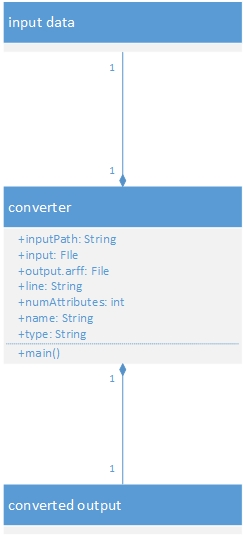
\includegraphics[scale=0.8]{UML.jpg}
\caption{UML Class Diagram for the converter}
\label{uml}
\end{figure}

\section{Design Decisions}
Python 2.7 was chosen for the converter because it provides a fast design to implementation life cycle. Furthermore the converter itself is a simple program, therefore it would be easier to understand in Python. The datasets which were chosen were based off of their lack of missing values and they present a range of attributes and instances for evaluation of the algorithms \citep{uci}. The datasets have attributes of size: $|a|=\{6,7,8,11,30\}$ and instances of size: $|i|=\{194,1728,4177,28056,1025010\}$. The names of the chosen datasets are: abalone, krkopt, car, flag, and poker-hand. Poker-hand does appear to be an outlier within $|i|$, so caution will need to be used if evaluations are made based on a certain algorithm across multiple datasets.

\pagebreak

\section{Experimental Design}
Each algorithm will be run using cross-validation with ten folds and then the different algorithms will be compared based on the data WEKA generates about time-elapsed, CPU use, false positive percentage, and false negative percentage. The five classification algorithms which will be evaluated are:
\begin{enumerate}
\item $K$-nearest neighbor (IBk) using $k>2$
\item Na\"ive Bayes
\item Logistic regression
\item Decision tree with pruning (J48)
\item Support vector machine with a nonlinear kernel (LibSVM)
\end{enumerate}

\pagebreak
\vskip 0.2in
\bibliography{references.bib}

\end{document}
